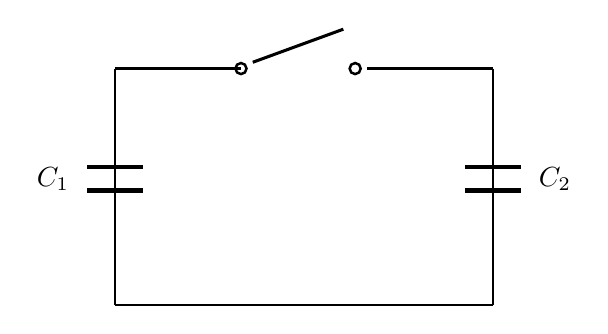
\begin{tikzpicture}[line width=0.9pt]
  % left wire down to C1
  \draw (0,0) -- (0,3.0);
  % top wire with open switch
  \draw (0,3.0) -- (1.6,3.0);
  \draw (1.6,3.0) circle (2pt);
  \draw[line width=1.1pt] (1.75,3.08) -- (2.9,3.5);
  \draw (3.05,3.0) circle (2pt);
  \draw (3.2,3.0) -- (4.8,3.0);
  % right wire down to C2
  \draw (4.8,3.0) -- (4.8,0);
  % bottom wire
  \draw (0,0) -- (4.8,0);
  % capacitor C1 (left, vertical plates)
  \draw[line width=1.6pt] (-0.35,1.75) -- (0.35,1.75);
  \draw[line width=1.6pt] (-0.35,1.45) -- (0.35,1.45);
  \draw (0,1.75) -- (0,3.0);
  \draw (0,0) -- (0,1.75);
  \node[left] at (-0.45,1.6) {$C_1$};
  % capacitor C2 (right, vertical plates)
  \draw[line width=1.6pt] (4.45,1.75) -- (5.15,1.75);
  \draw[line width=1.6pt] (4.45,1.45) -- (5.15,1.45);
  \draw (4.8,1.75) -- (4.8,3.0);
  \draw (4.8,0) -- (4.8,1.75);
  \node[right] at (5.25,1.6) {$C_2$};
\end{tikzpicture}
